\subsection{Sequence Diagram}

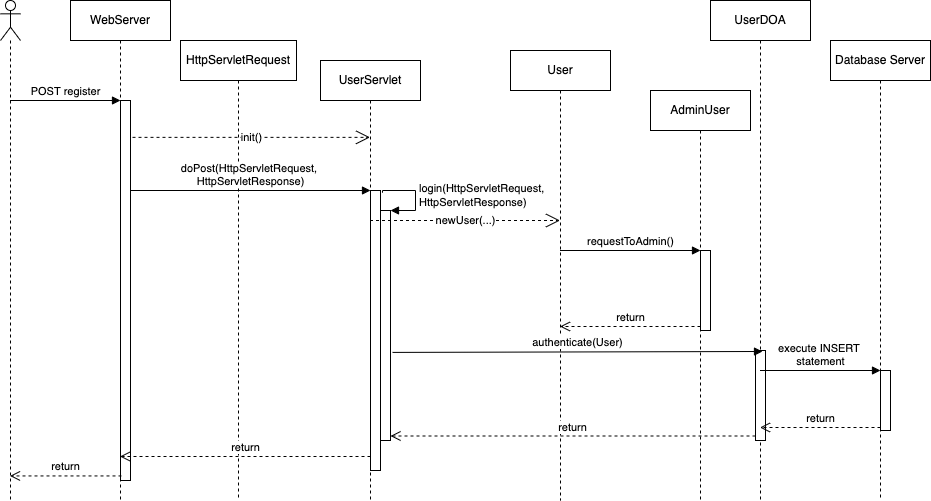
\includegraphics[]{figures/sequenceDiagram.png}

%describe here the sequence diagram

The sequence diagram shows how the registration of a new user.
The project uses the MVC pattern in the development.
User, AdminUser, UserDOA, and DatabaseServer are the models.
WebServer and HttpServletRequest interact as views, while UserServlet is the controller.
The sequence starts with a user that sends a POST request for registration to the WebServer.
A UserServlet is then initialised and executes methods for doPost() and login().
The user makes a call to the User model with newUser() and the User model asks for a request to the model AdminUser to approve the new user.
After the approval of the new user, the UserServlet sends an authenticate(User) to UserDOA for the model to INSERT the new user data into the DatabaseServer model.